
%Version 3 October 2023

\RequirePackage{amsthm}

\documentclass[sn-mathphys-num]{sn-jnl}% Math and Physical Sciences Numbered Reference Style 
%%\documentclass[sn-mathphys-ay]{sn-jnl}% Math and Physical Sciences Author Year Reference Style
%%\documentclass[sn-aps]{sn-jnl}% American Physical Society (APS) Reference Style
%%\documentclass[sn-vancouver,Numbered]{sn-jnl}% Vancouver Reference Style
%%\documentclass[sn-apa]{sn-jnl}% APA Reference Style 
%%\documentclass[sn-chicago]{sn-jnl}% Chicago-based Humanities Reference Style

%%%% Standard Packages
%%<additional latex packages if required can be included here>
\usepackage{rotating}
\usepackage{caption}
\usepackage{subcaption}
\usepackage{listings}
\usepackage{booktabs}
\usepackage{flushend}
\pagestyle{plain} %to show page numbers
\usepackage[most]{tcolorbox}
\usepackage[super]{nth}
\lstset{
basicstyle=\small\ttfamily,
columns=flexible,
breaklines=true
}
\usepackage{graphicx}%
\usepackage{multirow}%
\usepackage{amsmath,amssymb,amsfonts}%
\usepackage{amsthm}%
\usepackage{mathrsfs}%
\usepackage[title]{appendix}%
\usepackage{xcolor}%
\usepackage{textcomp}%
\usepackage{manyfoot}%
\usepackage{booktabs}%
\usepackage{algorithm}%
\usepackage{algorithmicx}%
\usepackage{algpseudocode}%
\usepackage{listings}%
\usepackage{lmodern}


% \newcommand{\todo}[1]{{\color{blue}$\blacksquare$~\textsf{[TODO: #1]}}}
%%%%%%%%%%%%%%%%%%%%%%%%%%%%%%%%%%%%%%%%%

%% as per the requirement new theorem styles can be included as shown below
\theoremstyle{thmstyleone}%
\newtheorem{theorem}{Theorem}%  meant for continuous numbers
%%\newtheorem{theorem}{Theorem}[section]% meant for sectionwise numbers
%% optional argument [theorem] produces theorem numbering sequence instead of independent numbers for Proposition
\newtheorem{proposition}[theorem]{Proposition}% 
%%\newtheorem{proposition}{Proposition}% to get separate numbers for theorem and proposition etc.

\theoremstyle{thmstyletwo}%
\newtheorem{example}{Example}%
\newtheorem{remark}{Remark}%

\theoremstyle{thmstylethree}%
\newtheorem{definition}{Definition}%

\raggedbottom
%%\unnumbered% uncomment this for unnumbered level heads

\begin{document}

\title[]{A Systematic Approach to Evaluating Development Activity in Heterogeneous Package Management Systems for Overall System Health Assessment} 

\author{\fnm{Shane K.} \sur{Panter}}\email{shanepanter@boisestate.edu}

\author{\fnm{Luke} \sur{Hindman}}\email{lukehindman@boisestate.edu}
%\equalcont{These authors contributed equally to this work.}

\author*{\fnm{Nasir U.} \sur{Eisty}}\email{nasireisty@boisestate.edu}
%\equalcont{These authors contributed equally to this work.}



%1910 W University Dr, Boise, ID 83725
\affil{\orgdiv{Department of Computer Science}, \orgname{Boise State University}, \orgaddress{\street{1910 W University Dr}, \city{Boise}, \postcode{83725}, \state{Idaho}, \country{USA}}}






%%==================================%%
%% Sample for unstructured abstract %%
%%==================================%%

\abstract{
\textbf{Context:}
Modern open-source operating systems consist of numerous independent packages crafted by countless developers worldwide. To effectively manage this diverse array of software originating from various entities, Linux distributions have devised package management tools to streamline the process. Despite offering convenience in software installation, systems like Ubuntu’s apt may obscure the freshness of its constituent packages when compared to the upstream projects. 
\textbf{Objective:}
The focus of this research is to develop a method to systematically identify packages within a Linux distribution that show low development activity between versions of the OSS projects included in a release. The packages within a Linux distribution utilize a heterogeneous mix of versioning strategies in their upstream projects and these versions are passed through to the package manager, often with distribution specific version information appended, making this work both interesting and non-trivial. 
\textbf{Method:}
We use regular expressions to extract the epoch and upstream project major, minor, and patch versions for more than 6000 packages in the Ubuntu distribution, documenting our process for assigning these values for projects that do not follow the semantic versioning standard. Using the libyears metric for the CHAOS project, we calculate the freshness of a subset of the packages within a distribution against the latest upstream project release. This led directly to the development of Package Version Activity Classifier (PVAC), a novel method for systematically assessing the staleness of packages across multiple distribution releases.
\textbf{Results:} 
We found that the heterogeneous nature of package versioning within a Linux distribution, as well as the lack of a standardized mechanism for determining the latest release of OSS projects, make calculating libyears infeasible for large numbers of packages. Using PVAC to look back at previous distribution releases did allow us to identify staleness and packages with little or no version activity across the evaluation period. While not a direct indicator of project health, the idea of staleness can be used to help identify OSS projects that need additional support or that have been orphaned.
\textbf{Conclusions:} We present a novel way to systematically evaluate the health of projects with heterogeneous package management systems, such as Ubuntu, by examining the staleness of its packages. The PVAC method we propose extends previous work by the software engineering research community by identifying packages with little to no development activity in the version of packages included within a distribution release.

}



\keywords{Open Source Software, Software Ecosystem, Health, Sustainability, Software Quality, CHAOSS, libyears}


\maketitle

\section{Introduction}
Linux is a widely used operating system, both here on earth as well as in space~\cite{vaughan-nichols_earth_2020}. This operating system, however, is not a single open-source project developed by a single team of open-source software developers. Instead, it is a collection of open-source software packages, each supported by various individuals or teams of open-source software developers, orchestrated by the Linux kernel. This collection of packages, bundled together with a Linux kernel, makes up a Linux distribution, which is what most people think of when it comes to the Linux operating system. 
% Because each individual package is updated independently and at different frequencies, we aim to use the libyears\footnote{https://chaoss.community/kb/metric-libyears/}~\cite{noauthor_metric_nodate} metric to assign a score to the whole distribution.

The modular architecture of a Linux distribution has enormous benefits and has enabled Linux to be deployed in everything from smartphones to spaceships~\cite{vaughan-nichols_linux_2023,vaughan-nichols_earth_2020}, from desktops to automobiles~\cite{vaughan-nichols_its_2019}, and everything in-between.  However, this modular architecture has an Achilles's heel: dependencies. Specifically, the health of the Linux distribution as a whole depends upon the health of all the constituent packages that make it up~\cite{linaker_how_2022}. In the past ten years, issues like the HeartBleed bug in OpenSSL (CVE-2014-0160)~\cite{noauthor_cve-2014-0160_2014}, ShellShock in BASH (CVE-2014-6271)~\cite{noauthor_cve-2014-6271_2014}, and more recently out-of-bounds memory access in GLIBCs qsort() (CVE-2023-6246)~\cite{noauthor_cve-2023-6246_2024} has lead to the creation of what is now known as the Open Source Security Foundation~\cite{noauthor_open_nodate}, allowing industry to more directly support the volunteers who maintain the core open source infrastructure. Aside from Android, Ubuntu and Debian comprise 49.9\% of the Linux~\cite{noauthor_linux_nodate} installation base with more than 6000 packages in the standard repositories. Hence, we chose to focus on the Ubuntu Linux distribution, which we feel would yield the most significant insights for our analysis.

% While using open-source software (OSS) can significantly reduce development costs, it also introduces some risks to the software engineering process. The maintenance of each open source component is typically delegated to the developer community~\cite{li_ossara_2022}, which may have health issues that are difficult to surface. Having a way to reliably measure the health and freshness of the system as a whole can help improve the quality of released OSS.

While using open-source software (OSS) can significantly reduce development costs, it also introduces some risks to the software engineering process. The maintenance of each open source project is typically delegated to the developer community~\cite{li_ossara_2022}, which may have health issues that are difficult to surface. In addition, OSS projects that are incorporated into a Linux Distribution are wrapped into packages that may no longer be actively maintained (staleness) or fall behind the latest available project releases (freshness). Having a way to systematically assess both the freshness and staleness of the packages within a Linux distribution will provide developers and maintainers better visibility into the underlying health of a particular distribution release.

The motivation for our research questions was to understand the health of a Linux distribution as a whole. Our research initially led us to the CHAOSS project~\cite{noauthor_metric_nodate}, where they described 89 different metrics for evaluating the health of OSS. By exploring these metrics, we found that the libyears\footnote{https://chaoss.community/kb/metric-libyears/}~\cite{noauthor_metric_nodate} metric is a good option to explore in part because it provides an objective means to assess the freshness of packages, and the data is readily available. However, we did not find a metric that examined staleness from the perspective of package maintenance activity across releases within a Linux distribution.  Therefore, we pose the following research questions:

\textit{\textbf{RQ1: Is it possible to classify the different versioning schemes used by packages in a Linux distribution?}}
This RQ aims to understand the types of versioning schemes used. While it would be helpful if every software project in the world used the same versioning scheme, each project has its own scheme. In order to derive the health of a package, we first need to surface all the different versioning methodologies. Admittedly this not a traditional research question, however, answering this question it is critical to our research to be able recognize the necessary version data so that we can effectively define inclusion/exclusion criteria in our later research.

\textit{\textbf{RQ2: Is it feasible to use the libyears version number delta to evaluate the freshness of the core Ubuntu packages?} }

The original work on the libyears~\cite{noauthor_metric_nodate} metric relied upon a homogeneous package management system where the versioning was consistent across packages. The first part of gauging feasibility is whether the libyears metric can provide useful information in a heterogeneous package management system. The second part of gauging feasibility is whether we can effectively calculate libyears for the packages listed in the Ubuntu core metadata package and, if so, scale it to the full 6000+ packages in the Ubuntu main package repository. 
% This RQ aims to calculate the libyears metric using the version number of the dependencies. We present a novel algorithm for calculating a single libyears number for a particular release.

\textit{\textbf{RQ3: Is there a systematic method to examine the staleness of packages within the Ubuntu main package repository?} }
% This RQ aims to find all the stale packages that are lurking in a package management system using the tools and dataset developed in \textbf{RQ1} and \textbf{RQ2}.
Similar to how the libyears metric examines freshness by comparing the version of a package or its dependencies against the latest upstream version release by the OSS project, we propose PVAC as a method to examine staleness by comparing the versions of packages within a particular Linux distribution release against the versions of the same packages in previous releases of the same distribution. Packages whose version show no difference in epoch, major, minor, and patch level between the releases, as well as those with only differences in patch level, are classified as sedentary or lightly active, respectively. In this work, we use PVAC to examine the packages in the Ubuntu 22.04 and 14.04 releases.

The main contributions of this paper are as follows:
\begin{itemize}
    \item We demonstrate that it is possible to classify package version data in a heterogeneous software repository. 
    \item We successfully performed a libyears analysis on a heterogeneous software repository, however we question the usefulness of this metric as an assessment of distribution health given the effort required to perform this analysis on even a minimal subset of packages.
    \item We propose PVAC, a novel method of systematically assessing distribution health by identifying stale packages with little to no development activity over multiple distribution releases. 
\end{itemize}


\section{Related Work}
Given the fact that OSS underpins large segments of modern society~\cite{miller_we_2023, goggins_open_2021, guizani_rules_2023}, significant research into how to measure the health of OSS, what to measure, how to report the results, and what actions to take have been conducted in recent years~\cite{noauthor_chaoss_nodate}. Research has been done on how to classify and categorize an OSS project in terms of both the project itself, the technical lag~\cite{decan2018evolution, gonzalez2017technical}, and its dependencies so developers can make informed decisions on the use of OSS components. Additionally, tools such as Augur~\cite{goggins_open_2021} have been created to help support both researchers and practitioners in analyzing the vast quantities of data available.

These efforts are only going to continue to grow due in large part to government requirements for creating secure and reliable software. For example, in 2021, the United States government signed an executive order on improving the nation's cybersecurity~\cite{house_executive_2021}. As part of that order, companies are required to provide a Software Bill of Materials (SBOM) to the requesting agency. A SBOM allows the consumer of a product to ensure all components are up-to-date and healthy so they can respond quickly to new vulnerabilities. While a list of all components used is a good start, we must also have a way to classify the health of said components.

Linaker et al.~\cite{linaker_how_2022} did a snowball literature review of publications about the health of OSS projects and found 107 health characteristics divided among 15 themes that can be used to characterize the health of OSS projects. They also confirmed how important it is not to analyze the OSS project in isolation. We must take into consideration its dependencies and ties to other projects to get a complete view of overall health.

Xiaozhou et al.~\cite{li_ossara_2022} developed the OSS Abandonment Risk Assessment (OSSARA) model to help companies assess the health of embedded OSS components. They used a classic risk assessment notion $Risk = Prob(Loss) \cdot Size(Loss)$ where they sum the risk of all OSS components in order to derive a risk score. The authors used data from GHTorrent to train a classifier that can predict the potential of a project being abandoned. The authors tested their solution on a real-world project and found positive reception when integrating the tool into an integration/continuous deployment pipeline.

The Linux Foundation has the significant motivation to ensure that OSS stays healthy and founded a working group, CHAOSS (Community Health Analytics in Open Source Software), in 2017. The CHAOSS project is focused on creating metrics, models, and software to better understand the health of OSS projects on a global scale~\cite{noauthor_chaoss_nodate}. This research is important because, as  Guizani at al.~\cite{guizani_rules_2023} found, ``companies want these projects [dependencies] to be healthy, alive and well maintained, and sustaining'' because it forms a core part of their day-to-day operations.

Miller et al.~\cite{miller_we_2023} researched how developers can prepare for the risk of OSS projects being abandoned and how to deal with the abandonment when it occurs. They conducted semi-structured, in-depth interviews with 33 developers who had experienced dependency abandonment to determine the best course of action. They found that the most common solution when dealing with dependency abandonment is to switch to a better-maintained alternative.

Cox et al.~\cite{cox_measuring_2015} studied project dependencies and their ``freshness''. They defined a metric to aid stakeholders in deciding if the dependencies of the project should be updated. They found that their metrics showed great potential in quantifying the dependency freshness of a system. The authors found that systems with a low dependency freshness score were four times as likely to contain security issues. Additionally, the authors conducted semi-structured interviews with five technical consultants at Software Improvement Group (SIG), and all interviewees considered the metric useful.

Our analysis of the related work found that a common thread among studies is it is important to have visibility into the health of all the components that comprise the system as a whole. While it may not be practical to measure all 107 health characteristics that Linaker et al.~\cite{linaker_how_2022} found or all 89 Metrics that the CHAOSS~\cite{noauthor_chaoss_nodate} project defined, there was universal agreement that some metric and data collection is necessary.

% \begin{figure*}
%     \centering
%     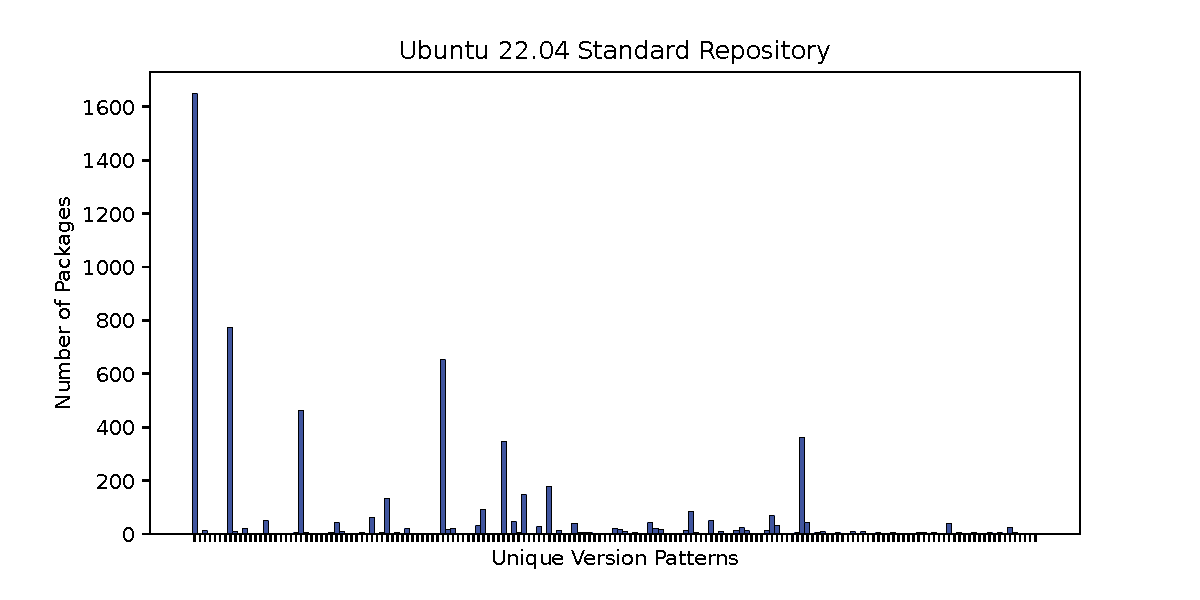
\includegraphics[width=7in]{figures/basic-class-histogram.pdf}
%     \caption{Basic Package Distribution}
%     \label{fig:basic-class-histogram}
% \end{figure*}

\section{Data}
In this section, we describe our research dataset, including relevant background information. 

 \begin{figure*}
    \centering
     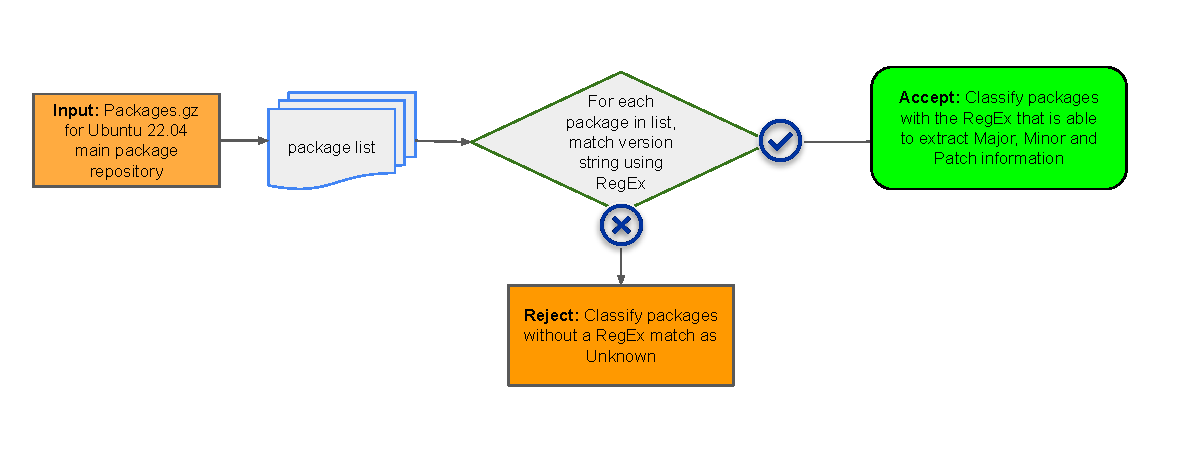
\includegraphics[width=\columnwidth]{figures/process-diagram-RQ1.pdf}
     \caption{Process Diagram for RQ1}
     \label{fig:process-rq1}
 \end{figure*}

 \begin{figure*}
    \centering
     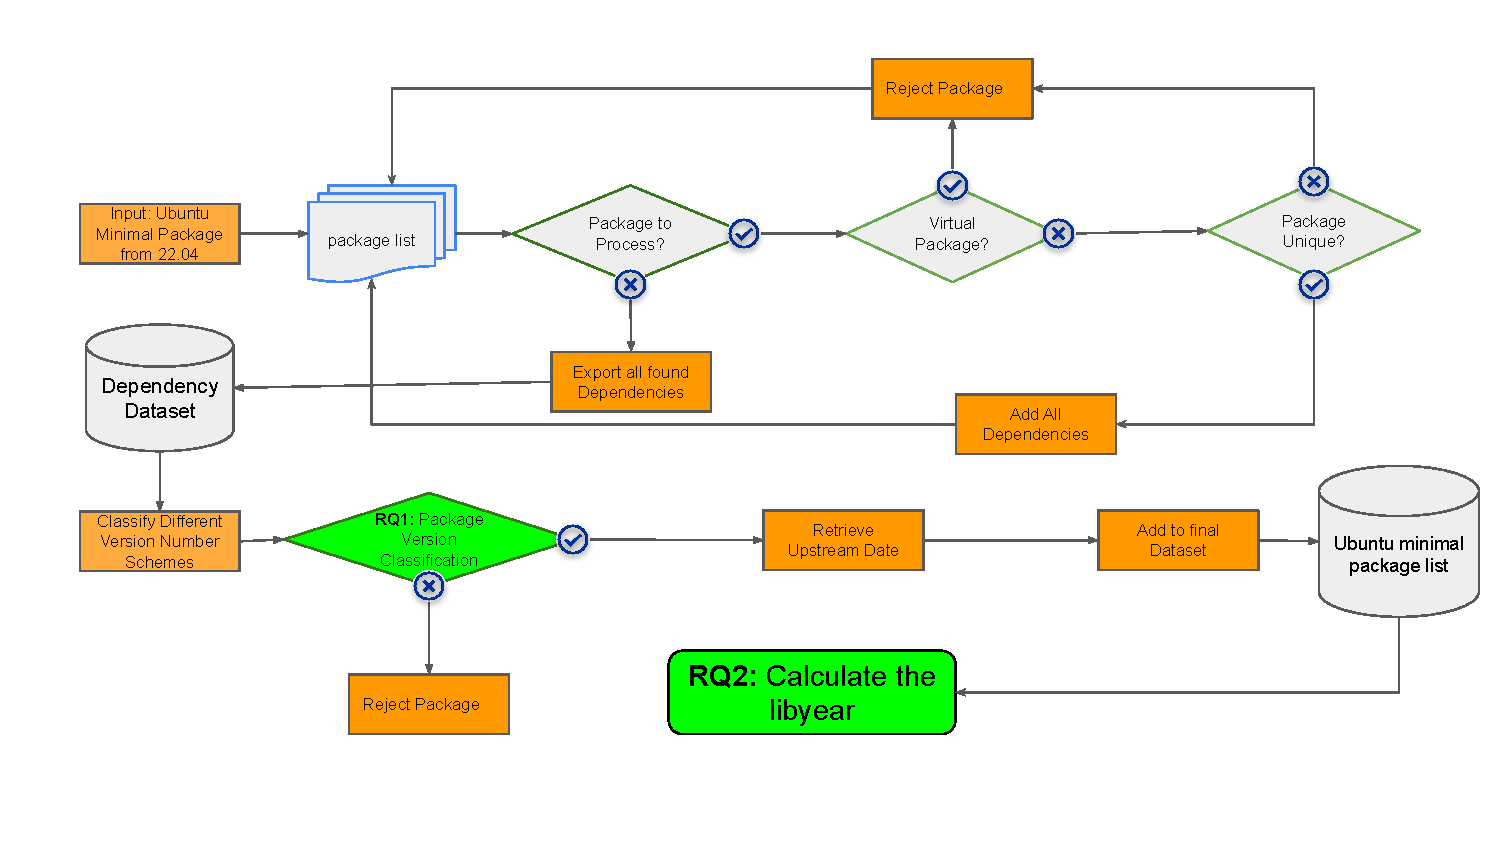
\includegraphics[width=\columnwidth]{figures/process-diagram-RQ2.pdf}
     \caption{Process Diagram for RQ2}
     \label{fig:process-rq2}
 \end{figure*}


 \begin{figure*}
    \centering
     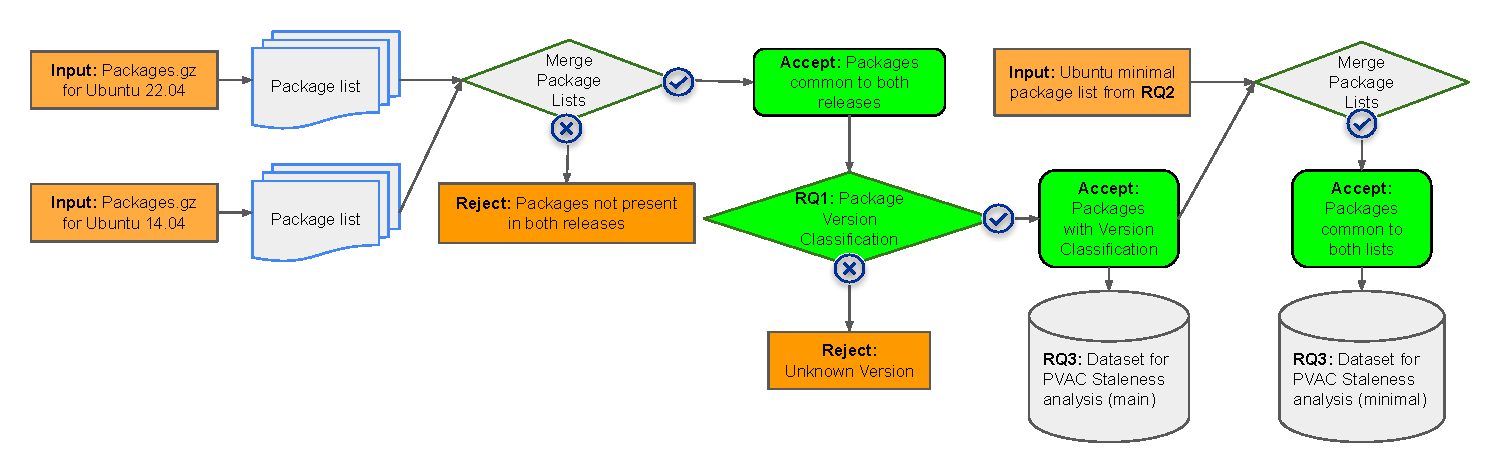
\includegraphics[width=\columnwidth]{figures/process-diagram-RQ3.pdf}
     \caption{Process Diagram for RQ3}
     \label{fig:process-rq3}
 \end{figure*}

\subsection{Libyears}
 
We used a health metric called libyears~\cite{cox_measuring_2015}, which provides an assessment of how ``fresh'' a project is by examining how out-of-date the dependent packages are compared to the latest stable versions. 
Libyears was defined by Cox et al.~\cite{cox_measuring_2015} and is now a part of the CHAOSS project. Calculating the libyears can be done multiple ways, not only with the date of the package but also with the version number delta. 

The original implementation was performed within a homogeneous package system (Maven) and only a single programming language (Java). As stated by the CHAOSS project, ``By default, this information will be within an ecosystem (e.g., JavaScript or Maven), as that is easier to compute''~\cite{noauthor_metric_nodate}. Unfortunately, Linux distributions do not have uniform version scheme, language, or upstream package structure, so in order to leverage libyears in evaluating the health of a Linux distribution, we classify the various versioning schemes and create a mapping to extract the necessary epoch, major, and minor data from each package's version string, manually research the upstream dates to verify our process and finally invent a novel way to calculate the libyears from that data.

\subsection{Dataset}
To construct the dataset necessary to do the experiments, first, we gathered the package data, then we extracted the dependencies, annotated them with version number type, and finally manually derived the upstream dates of the packages as detailed in figures~\ref{fig:process-rq1},~\ref{fig:process-rq2}, and~\ref{fig:process-rq3}.

The package data for the main Ubuntu repositories is provided in a file named Packages.gz that can be downloaded from the respective release archive, for example, 22.04 (jammy)~\cite{noauthor_index_nodate}. When decompressed, we have a text document that provides detailed package data for the more than 6000 packages in the distribution. We developed a Python script to do a depth-first search of the package hierarchy to extract all the dependencies and a subset of the control fields for each package. We filtered out all virtual packages as they are just a construct of the package management system itself, as well as packages that were unique to just one distribution because new packages would always be fresh when they are first added into the distribution. 

Once we had the initial set of dependencies, we extracted all packages with compatible version number schemes. Clearly, we can not calculate the libyears delta between two packages that are using mutually exclusive version numbers. In order to classify each package as version number delta compatible, we used regular expressions to identify and tag each package with a group ID based on a pattern match. These patterns are composed of strings of numbers ([0-9]+), strings of letters ([a-z]+), and delimiters (.,+,-,\textasciitilde). For this initial classification step, we intentionally did not use more complex regular expressions so we could better identify the components within each version string. For the first pass, we found 141 packages from 20.04 LTS and 158 packages from 22.04 LTS, bringing down the package count from more than 6000 packages. Finally, we further limited the dataset to the ubuntu-minimum dataset, which is the set of packages that must be included for the system to be functional and can not be removed. The final dataset contained 99 packages and is the dataset that we will use to derive the upstream dates of the source code from which the Ubuntu packages are built.

We made our dataset and artifacts available at - 

https://figshare.com/s/6486c76356e496171db6.


\section{Experiments and Results}
This section presents our analysis and findings of examining the health of a subset of the Ubuntu package. 

\subsection{\textbf{RQ1: Is it possible to classify the different versioning schemes used by packages in a Linux distribution?}}
While the goal of this research is to evaluate the freshness/staleness of the Ubuntu distribution packages, we first have to determine the current state of version numbering within the Ubuntu package management system. For this particular research question, we examine the full set of more than 6000 packages in the standard Ubuntu 22.04 (jammy) main repository to ensure we have a good characterization of the various versioning schemes, as shown in figure~\ref{fig:process-rq1}. 

\subsubsection{\textbf{Basic Classification}}


This initial classification was performed on the 6000+ packages stored within the main Ubuntu 22.04 repository. Of these packages, 167 unique version formats were found, with regular expressions manually constructed for each. The distribution of packages across these unique version formats is quite sparse, with the \nth{50} quantile only matching three packages and the \nth{90} quantile matching only 43 packages. The most common version format is shown in Listing~\ref{lst:common_version} with 1648 packages using this format. 

% Figure \ref{fig:basic-class-histogram} shows this sparse distribution visually.

\begin{lstlisting}[caption={Most Common Version Format},captionpos=b, label=lst:common_version]

1.1.1-1ubuntu1  

\end{lstlisting}



\subsubsection{\textbf{Semantic Classification}}

\begin{figure*}[htbp]
    \centering
    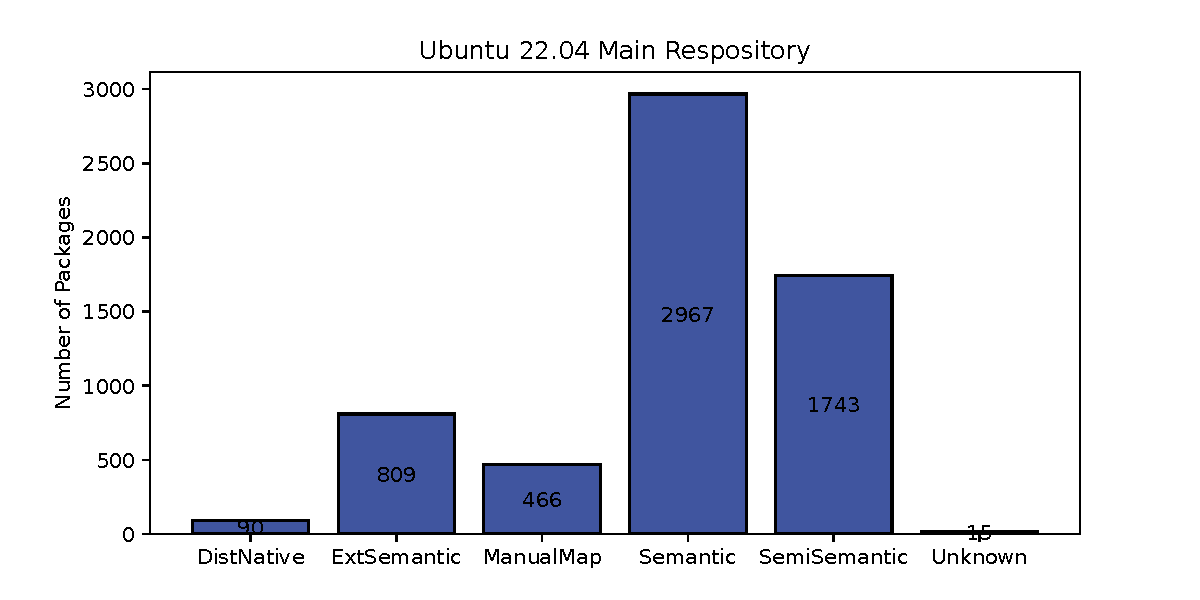
\includegraphics[width=\columnwidth]{figures/semantic-class-histogram.pdf}
    \caption{Semantic Package Distribution}
    \label{fig:semantic-class-histogram}
\end{figure*}

Our analysis of the basic classification results revealed a number of common patterns that could easily be combined into a single regular expression. Next, we found that nearly half of the packages in our dataset conformed to the semantic versioning standard~\cite{preston-werner_semantic_nodate}. The official documentation for the semantic versioning standard provides an official regular expression (RegEx) for recognizing version strings correctly formatted using semantic versioning as shown in listing~\ref{lst:regular_expression}.

\begin{lstlisting}[caption={Semantic Version Regular expression},captionpos=b, label=lst:regular_expression]
^(?P<major>0|[1-9]\d*)\.(?P<minor>0|[1-9]\d*)\.(?P<patch>0|[1-9]\d*)(?:-(?P<prerelease>(?:0|[1-9]\d*|\d*[a-zA-Z-][0-9a-zA-Z-]*)(?:\.(?:0|[1-9]\d*|\d*[a-zA-Z-][0-9a-zA-Z-]*))*))?(?:\+(?P<buildmetadata>[0-9a-zA-Z-]+(?:\.[0-9a-zA-Z-]+)*))?$
\end{lstlisting}

To test this, we placed the above RegEx as the first in the match set. Any version strings that did not align with the official semantic RegEx fell through to the basic classifier. From these results, we now have a single semantic classification group that contains 2967 packages. By using named groups in our regular expressions, we are able to easily extract the data necessary for the libyears analysis from packages that are successfully classified.

\subsubsection{\textbf{Extended Semantic Classification}}

The Debian Policy Documentation~\cite{noauthor_5_nodate} defines the requirements for distributions that use the Debian package management system. This policy described an optional \textbf{epoch} value that can be pretended as well as an optional \textbf{debian\_revision} that can be appended, encapsulating the original upstream version information. The standard format is shown in listing~\ref{lst:debian_upstream}.

\begin{lstlisting}[caption={Debain Extended Version Format},captionpos=b, label=lst:debian_upstream]
[epoch:]upstream_version[-debian_revision].
\end{lstlisting}

From the Debian versioning policy: ``[Epoch] is a single (generally small) unsigned integer. It may be omitted, in which case zero is assumed. When comparing two version numbers, first the epoch of each is compared, then the upstream\_version if epoch is equal, and then debian\_revision if upstream\_version is also equal.''~\cite{noauthor_5_nodate}

The ExtendedSemantic classification checks for the prepended epoch value at the head of an otherwise Semantic version string. Based upon the Debian versioning policy, the Semantic classification would also be considered ExtendedSemantic, with the epoch of 0 omitted. For upstream\_versions that followed the Semantic versioning standard, the Debian revision tags were properly matched using the Semantic versioning RegEx.

Applying the ExtendedSemantic classification (ExtSemantic), we could classify an additional 809 packages.

\subsubsection{\textbf{SemiSemantic Classification}} 

An examination of the remaining packages indicated that if certain requirements of semantic versioning were relaxed, we would likely be able to classify a significant number of additional packages. To that end, we made the following adjustments to the ExtendedSemantic regular expression:

\begin{enumerate}
    \item Allow version numbers with leading zeros, such as 001
    \item Make the patch field optional. Packages without patch fields are assigned a patch value of 0
    \item Recognize patch fields that are separated from the minor field by either a `.' or a lowercase `p' or `pl'
\end{enumerate}

Applying the SemiSemantic classification (SemiSemantic), we were able to extend our classification by 1743 additional packages further.

\subsubsection{\textbf{Distribution Native Classification}}

The Debian Mentors FAQ describes the two types of packages in a Debian Linux system and its derivatives: native and non-native~\cite{noauthor_debianmentorsfaq_nodate}. The majority of packages in the Ubuntu distribution are non-native, meaning 3rd parties maintain them and may be used by a variety of Linux distributions. The distribution maintainers maintain packages with native versioning and are only useful inside the Debian / Ubuntu ecosystem. 

The version format for Debian native packages is similar to SemiSemantic, but the trailing \textbf{-debian\_version} is removed. If this were the only change, this would be fairly simple to classify.  However, for Ubuntu native packages, often only the hyphen is removed, and the remainder of the tag is appended directly to the \textbf{upstream\_version} portion without the delimiter.  

Applying the Distribution native classification (DistNative), we were able to classify and extract the necessary data from an additional 90 packages.

\subsubsection{\textbf{Manual Classification}}
The remaining packages contain valuable version data necessary for our libyears analysis. However, the version patterns were structured in such a way that they did not conform to our previous classification efforts. We manually created individual regular expressions, classifying small groups of packages to provide access to the necessary major, minor, and patch fields. The following accommodations were made to preserve as much packaging information as possible for our libyears analysis.

\begin{enumerate}
    \item If the patch field is missing, a patch value of 0 is assigned
    \item If the minor field is missing, a minor value of 0 is assigned
    \item If the epoch field is missing, an epoch value of 0 is assigned.
\end{enumerate}

A recognizable major version field is the only field that is absolutely required for Manual classification (ManualMap). Using this strategy, we were able to classify 466 additional packages.

\subsubsection{\textbf{Unknown Classification}}

The Unknown classification was used for packages with no immediately recognizable major version field that was suitable for our libyears analysis. In some cases, this is simply a date, and in others, it is a version control commit ID. Of the more than 6000 packages in the Ubuntu 22.04 main repository, only 15 received the Unknown classification.

\begin{figure}[h]
    \centering
    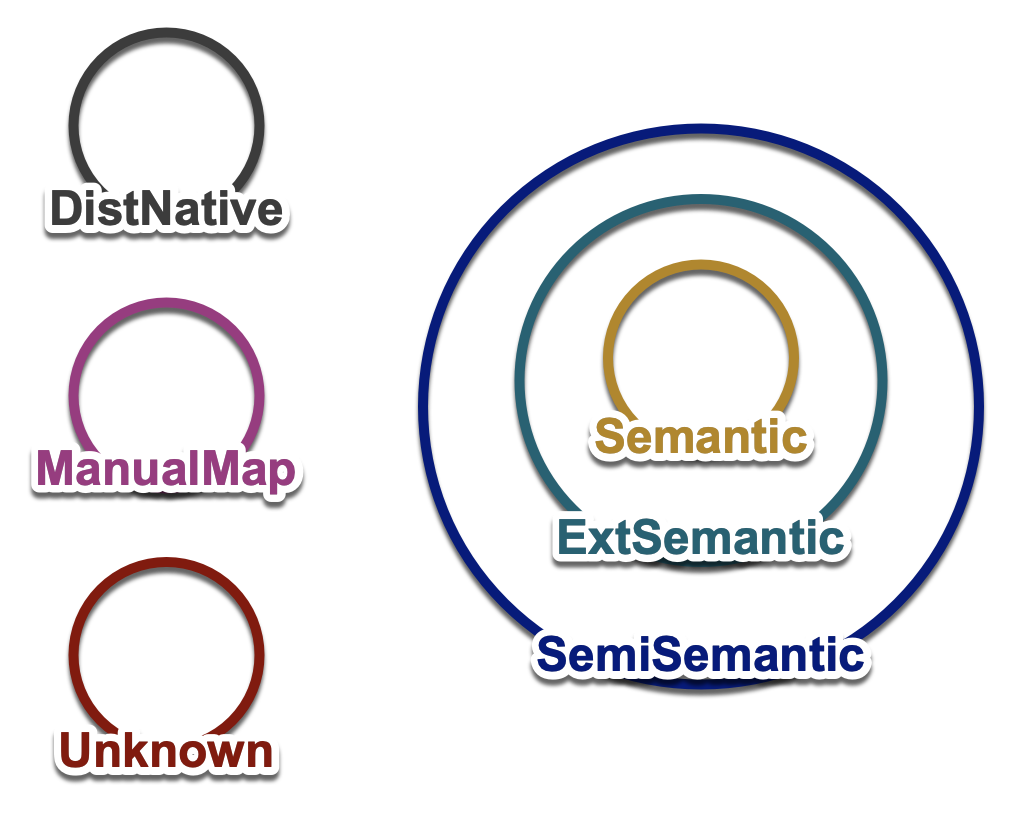
\includegraphics[width=0.75\linewidth]{figures/package-classes.png}
    \caption{Package Classes}
    \label{fig:class-relationships}
\end{figure}

Both the libyears delta version analysis and the PVAC analysis require the major, minor, and patch data provided with the semantic versioning. The SemiSemantic class provides these required fields, and figure~\ref{fig:class-relationships} shows the relative relationship between the package version classes with SemiSemantic encapsulating both ExtSemantic and Semantic classes with the DistNative and ManualMap classes being disjoint from the Semantic classes. It would have been possible to incorporate DistNative into SemiSemantic, however it would have required more extensive adjustments to the SemiSemantic class and keeping it disjoint provides an interesting view of distribution maintained packages vs external packages. Figure~\ref{fig:semantic-class-histogram} shows the overall distribution of the version class of the 6000+ packages in the Ubuntu 22.04 main repository.

\begin{tcolorbox}[enhanced,attach boxed title to top center={yshift=-3mm,yshifttext=-1mm}, colback=blue!5!white,colframe=blue!75!black,colbacktitle=red!80!black, title=Answer to RQ1,fonttitle=\bfseries, boxed title style={size=small,colframe=red!50!black} ]

   We successfully classified 6075 of the Ubuntu packages in the main repository, creating regular expressions to extract the epoch, major, minor, and patch data necessary for performing both the libyears delta version and PVAC analysis.

\end{tcolorbox}

\subsection{\textbf{RQ2: Is it feasible to use the libyears version number delta to evaluate the freshness of the core Ubuntu packages?}}

The paper~\cite{cox_measuring_2015} that introduced the libyears metric for evaluating the freshness of OSS packages described several different methods of calculating the libyears of a system. One method uses the Major.Minor.Patch version data to calculate a version delta, while another method uses the release date. For this research question, we explored the possibility of calculating the libyears using the version delta technique described by Cox et al.~\cite{cox_measuring_2015}.  Figure~\ref{fig:process-rq2} outlines our process for this research question. 

Given the wide variety of versioning schemes identified in RQ1, the question we must consider is whether we have sufficient versioning information to perform a libyears analysis of the core Ubuntu packages. Our results in RQ1 revealed that less than 1\% did not contain sufficient version data to perform that analysis, and we excluded those packages. Figure~\ref{fig:class-by-release} shows the distribution of these packages across the classes identified in RQ1.

\begin{figure*}[h]
    \centering
    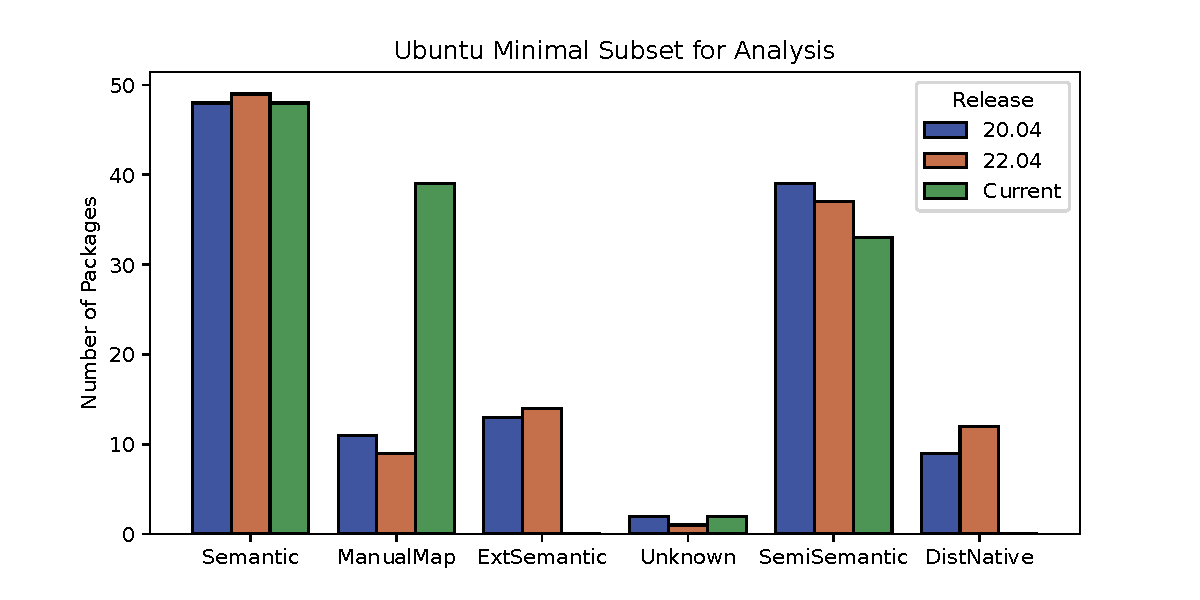
\includegraphics[width=\columnwidth]{figures/class-distribution-by-release.pdf}
    \caption{Class Distribution by Release}
    \label{fig:class-by-release}
\end{figure*}

\subsubsection{\textbf{Libyears Analysis Using the Version Number Delta}}
\label{sec:vnd}

%Given the wide variety of versioning schemes identified in RQ1, the question we must consider is whether we have sufficient versioning information to perform a libyears analysis of the core Ubuntu packages. Thankfully, our work in RQ1 has revealed only three packages did not contain sufficient version data to perform that analysis and those packages have been excluded from this dataset. 
We excluded all virtual and meta packages as well as any package that did not have an upstream source listed. To perform our libyears calculations, we selected all packages in the \textbf{ubuntu-minimal} set with valid semantic versions, a valid homepage for the upstream package, and not a virtual or meta-package, leaving a grand total of 99 packages to work with. The \textbf{ubuntu-minimal} meta package is the set of packages that are fundamental to the system as a whole and are thus the most important packages to keep fresh.

As detailed by Cox et al.~\cite{cox_measuring_2015}, there are a few issues with using the version number delta to calculate the libyears. First, there is no meaningful way to aggregate all the tuples together due to the extreme variability between projects and how they assign the version tuple. We confirmed this statement when we were constructing the dataset, collecting upstream dates, and confirming upstream version numbers. Some projects that we examined did, in fact, have a documented method for incrementing the version number~\cite{noauthor_versioning_2017} while other projects versioned the numbers based on the ``feeling'' of the lead developer~\cite{noauthor_interview_2021}, while still, others had no documented process on how their packages were versioned at all. Our findings confirmed Decan et al.~\cite{decan2019package} that only a meticulous
analysis of the semantics of the code can allow the users to assess its compatibility across semantic versions. Despite these shortcomings, we believe that calculating the libyears based on the version sequence number has value because getting the version number of a package is infinitely more accessible than trying to derive the upstream date and deriving the date off of the package itself varies between Linux distributions. Thus, using the version number allows a more accurate comparison between Linux distributions that may have different ways of handling the dates of the packages themselves.

We propose a meaningful way to calculate a single number using the Version Number Delta and then compare the results using the upstream package dates. We propose calculating the libyears using the semantic version numbers by expressing the semantic version as a single number using the following formula $libyear = (major * .7) + (minor * .20) + (patch *.10)$. Each component of the semantic version was weighted based on is perceived impact on compatibility between components. As specified by the semantic version specification~\cite{preston-werner_semantic_nodate} ``the major number should be incremented when you make incompatible API changes, the minor version should be incremented when you add functionality in a backward compatible manner, and the patch version should be incremented when you make backward compatible bug fixes.'' Thus, we will weigh each part of the semantic version with a value that represents how big of an impact a change has, 70\% for the major version, 20\% for the minor version, and 10\% for the patch version. With this formula, we can now calculate the libyears of the dataset constructed from Ubuntu 20.04 and 22.04., as shown in table~\ref{tab:libyear}.


\begin{table}[h]
    \centering
    \begin{tabular}{|c|c|c|} \hline 
         Ubuntu LTS Version&  Libyears Version Delta& Libyears Upstream Date  \\ \hline 
         20.04&  53.89& 68362 Days \\ \hline 
        22.04& 15.86&44496 Days \\\hline
    \end{tabular}
    \caption{Libyear for ubuntu-minimal}
    \label{tab:libyear}
\end{table}

\begin{table}[htbp]
    \centering
    \begin{tabular}{lllllll}
    \toprule
    package & Class & major & minor & patch & upstream\\
    \midrule
    perl-base & Semantic & 5 & 38 & 2 & 11/29/23 \\
    e2fsprogs & Semantic & 1 & 47 & 0 & 2/7/23 \\
    logsave & Semantic & 1 & 47 & 0 & 2/7/23  \\
    libgcc-s1 & SemiSem & 13 & 2 & 0 & 7/27/23 \\
    libstdc++6 & SemiSem & 13 & 2 & 0 & 7/27/23 \\
    libcap-ng0 & Semantic & 0 & 8 & 4 & 12/20/23 \\
    less & ManualMap & 643 & 0 & 0 & 8/12/23  \\
    libapparmor1 & Semantic & 3 & 0 & 13 & 2/2/24  \\
    libgcrypt20 & Semantic & 1 & 10 & 3& 11/14/23 \\
    liblz4-1 & Semantic & 1 & 9 & 4 & 8/15/22 \\
    libzstd1 & Semantic & 1 & 5& 5 & 4/4/23 \\
    \bottomrule
    \end{tabular}
    \caption{Sample Data from the Constructed Upstream Dataset}
    \label{tab:upstream_data}
\end{table}

\subsubsection{\textbf{Libyears Analysis Using Release Date}}

Using the libyears version delta, we can clearly see that newer distributions have a lower value, meaning they are fresh. To verify that this data is meaningful, we compared the libyears version delta to the libyears calculated from the upstream date. Measuring the distance between two releases of a dependency based on the date the package was released should also yield an increasing number as we get further and further from the current version. Damien et al.~\cite{legay_quantitative_2021} looked at the package freshness in Linux distributions using this method. However, they used the package date of the distribution itself instead of the date from the upstream source. Damien et al. found no aggregate source of information on upstream release dates, which we confirmed. Despite there being no existing data sources for upstream packages, we still wanted to look at a minimal subset of the full 6000+ packages and calculate the libyears based on the upstream date. We took the data set constructed for section~\ref{sec:vnd} and derived upstream dates for all packages in that data set.

It took one researcher approximately 16 hours to manually find the upstream release date of each package. Table~\ref{tab:upstream_data} shows a sample of the constructed dataset with each package classified with its versioning scheme, its major, minor, and patch version extracted, as well as the upstream date of the released code. Not every upstream dependency had a clear correlation between the version number and the date it was released, so we used a standardized process to determine the date. While this may have resulted in an incorrect date-to-version pairing for some packages, it was the only option considering the variability between projects in such a diverse system as Ubuntu packages.
First, if the upstream had a website with a post announcing the version that date was used first. Second, if the upstream released their code on an FTP or file server, that date was used. Third, for packages that were hosted on GitHub or GitLab and used the release features, that date was used. Finally, the date was determined by cloning the repository and either looking for a version control tag or some file in the repository itself indicating the exact date that the version number was released.

We defined a new method to calculate the libyears based on the version number delta. While making a direct comparison against the Version Release Date does not have much meaning in itself, we do find that both metrics show an increasing libyears value on older releases, which is to be expected. So, while we may not be able to directly compare the different libyears calculation functions, we are confident that our suggested approach to calculating a single value using the Version Number Delta can provide another view of the data when the dates are difficult, if not impossible, to get.

\begin{tcolorbox}[enhanced,attach boxed title to top center={yshift=-3mm,yshifttext=-1mm}, colback=blue!5!white,colframe=blue!75!black,colbacktitle=red!80!black, title=Answer to RQ2,fonttitle=\bfseries, boxed title style={size=small,colframe=red!50!black} ]

   We successfully calculated a single value representing the libyears of a project using the version number alone. Our research shows that as we go back further in time, our method correctly produces larger and larger values as code gets more and more out of date. However, the challenges involved in locating and manually collecting release data for the upstream OSS projects for even a small subset (\textless2\%) of the packages in the Ubuntu package repository make this analysis infeasible to perform on the full 6000+ packages.

\end{tcolorbox}

\subsection{\textbf{RQ3: Is there a systematic method to examine the staleness of packages within the Ubuntu main package repository?}}

When examining the freshness of the Ubuntu distribution in RQ2, we calculated the libyears by comparing the package versions and release dates of Ubuntu 20.04 (focal) and 22.04 (jammy) against the latest upstream release. Unfortunately, this approach was extremely time-intensive, given that the upstream versions and release dates had to be manually collected, limiting the number of packages we could examine. In addition, we found that we could not directly compare version number delta values in a meaningful way. 

Our goal with this research is to examine the overall health of a Linux distribution by identifying packages that have been orphaned or are no longer being actively developed and maintained. While the the libyears metric calculated with the version number delta did give us a global view of the health of the system, we also wanted to drill down into individual packages so we can find specific issues within the system as a whole. For this research question, we propose the Package Version Activity Classifier (PVAC) as a systematic method for assessing the upstream development activity of packages across Ubuntu releases. PVAC takes the version strings for the same package across two different Ubuntu releases and compares them. Figure~\ref{fig:process-rq3} outlines our process for this research question.

\begin{table}[h]
    \centering
    \begin{tabular}{p{0.25\linewidth} p{0.5\linewidth}}
    \toprule
         Activity Level & Description \\ 
    \toprule
         Major Change & Difference found in major version\\
         Moderately Active & Matching major version, but difference found in minor version \\ 
         Lightly Active & Matching major and minor versions, but difference found in patch version \\ 
         Sedentary & Matching major, minor, and patch versions \\ 
        \bottomrule
    \end{tabular}
    \caption{PVAC Activity Classification}
    \label{tab:pvac_activity_classificaiton}
\end{table}

Based upon the Debian Versioning Policy, it is only valid to compare versions with the same epoch. If the upstream major version is different between the two versions, PVAC classifies the package as \textbf{Major Change} over the time period between the two Ubuntu releases. If the upstream major version is the same, but the minor version has changed, PVAC classifies the package as \textbf{Moderately Active} over the evaluation period. If the upstream major and minor versions are identical, but the patch level has changed, PVAC classifies the package as \textbf{Lightly Active}.  And finally, if the upstream major, minor, and patch versions are identical for both releases, with only Debian or Ubuntu packaging changes, the package is classified as \textbf{Sedentary}. Table \ref{tab:pvac_activity_classificaiton} provides a more concise description of the PVAC Activity Classifications. Listing \ref{lst:pseudo_pvac} shows a pseudocode implementation of the PVAC classification method.

\begin{lstlisting}[language={Python}, caption={Pseudocode implementation of PVAC}, label={lst:pseudo_pvac}]
def pvac(pkg_R1,pkg_R2):

    sem_R1 = lookup_sem_class(pkg_R1)
    sem_R2 = lookup_sem_class(pkg_R2)
    
    if sem_R1['epoch'] != sem_R2['epoch']:
        return None
    
    activity_level = "Sedentary"
    
    if sem_R1['major'] != sem_R2['major']:
        activity_level = "Major Change"
    elif sem_R1['minor'] != sem_R2['minor']:
        activity_level = "Moderately Active"
    elif sem_R1['patch'] != sem_R2['patch']:
        activity_level = "Lightly Active"

    return activity_level
\end{lstlisting}


\subsubsection{\textbf{Evaluating PVAC on Ubuntu Main Repository}}
In order to evaluate the effectiveness of PVAC as a tool to evaluate the staleness of packages in Ubuntu systematically, we compared packages in the Ubuntu main repository from the 14.04 (trusty) release and the 22.04 (jammy) releases. Figure~\ref{fig:ubuntu-release-package-count} shows the Ubuntu Release Package Count for the 22.04 and 14.04 releases with 6090 and 8566 packages, respectively. PVAC is only suitable to use on the 3357 packages in common between the two releases, so this is our working data set.

% \begin{figure*}[h]
%     \centering
%     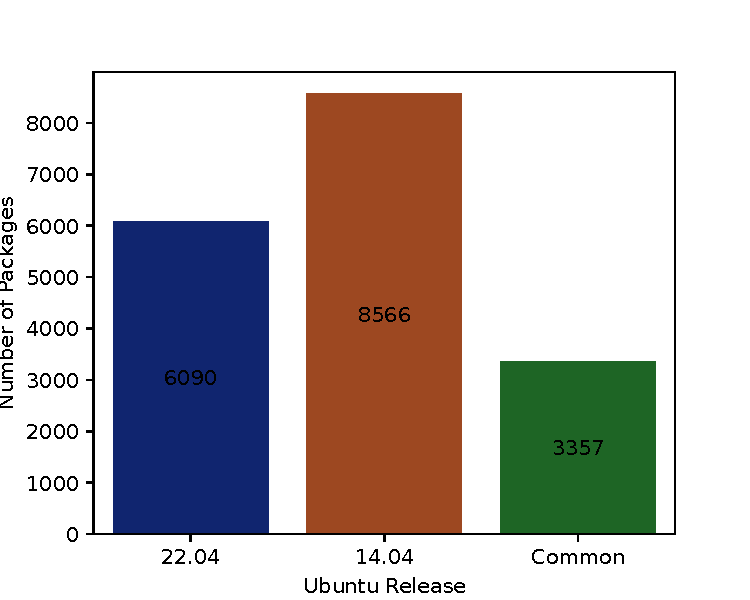
\includegraphics[width=7in]{figures/ubuntu-release-package-count.pdf}
%     \caption{Ubuntu Release Package Count}
%     \label{fig:ubuntu-release-package-count}
% \end{figure*}
\begin{figure}
    \centering
    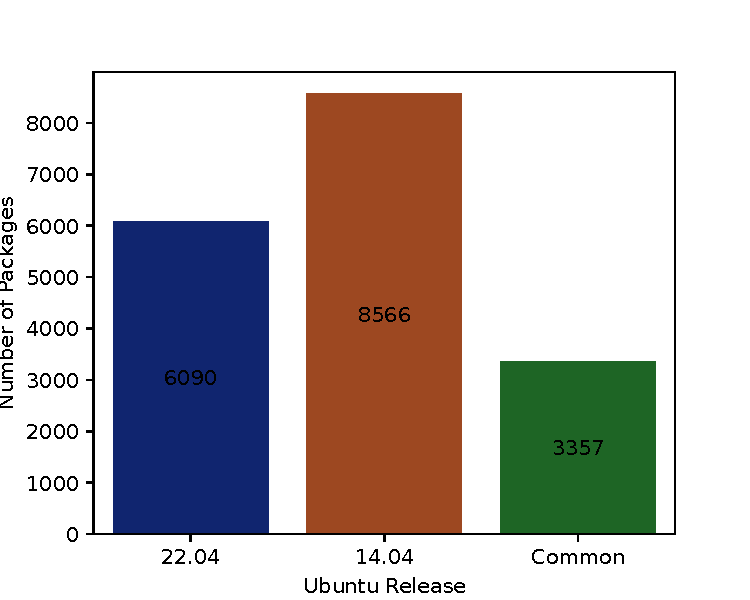
\includegraphics[width=1.0\linewidth]{figures/ubuntu-release-package-count.pdf}
    \caption{Ubuntu Release Package Count}
    \label{fig:ubuntu-release-package-count}
\end{figure}


\begin{figure}
    \centering
    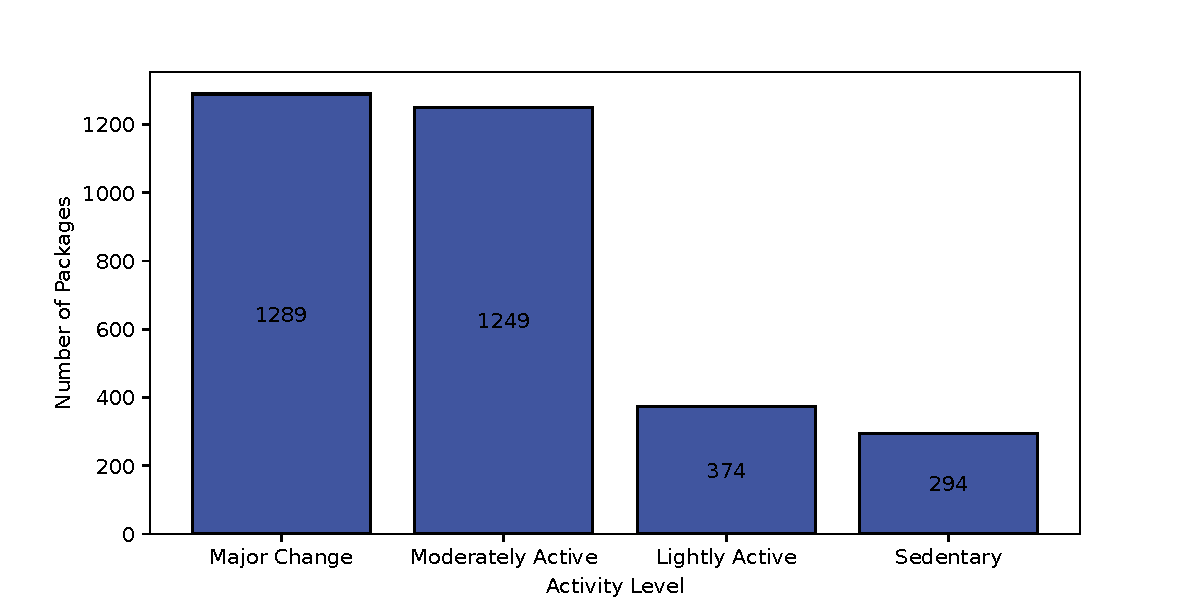
\includegraphics[width=1.0\linewidth]{figures/ubuntu-release-package-activity-main.pdf}
    \caption{Ubuntu Release Package Activity (main repository)}
    \label{fig:ubuntu-release-package-activity-main}
\end{figure}

Next, we classified the common packages in the 14.04 and 22.04 releases using the process developed in RQ1 to ensure we can extract the necessary epoch, major, minor, and patch version information. We excluded packages that do not exist in both repositories or that do not both provide the necessary data. Approximately 2.7\% of the common packages were classified as Unknown, leaving 3266 packages for the PVAC analysis.

% Figure \ref{fig:ubuntu-release-package-classification} shows the Ubuntu Release Package Classification with
%  Disabled to make write-up more concise
% \begin{figure}
%     \centering
%     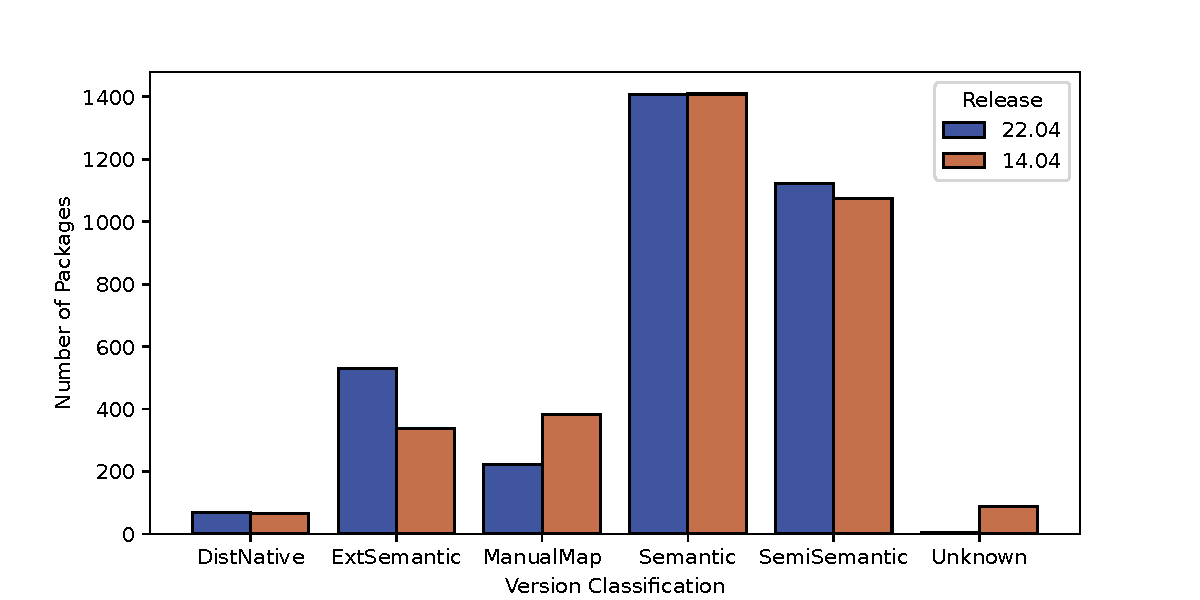
\includegraphics[width=1.0\linewidth]{ubuntu-release-package-classification.pdf}
%     \caption{Ubuntu Release Package Classification}
%     \label{fig:ubuntu-release-package-classification}
% \end{figure}


Figure~\ref{fig:ubuntu-release-package-activity-main} shows the Ubuntu Release Package Activity generated by PVAC over the eight-year period between the 14.04 and 22.04 releases, with 374 packages being classified as \textbf{Lightly Active} and 294 packages classified as \textbf{Sedentary}. As mentioned earlier, this analysis is across the packages in the main repository for the respective releases.


\subsubsection{\textbf{Evaluating PVAC on Ubuntu Minimal Dataset from RQ2}}
Tightening the focus even further, we performed the PVAC analysis on the Ubuntu Minimal dataset from RQ2. Figure~\ref{fig:ubuntu-release-minimal-metadata-package-activity} shows the results for these packages, which are common across the majority of Ubuntu installs. This analysis shows that there are 8 \textbf{Lightly Active} packages and 1 \textbf{Sedentary} package over that 8-year period between releases. Table~\ref{tab:sedentary-packages} lists these nine packages identified by PVAC. 

While this dataset has substantially fewer packages than the main, it demonstrates the utility of the PVAC. The listing of packages that are Lightly Active or Sedentary provides an excellent starting point for assessing the staleness of packages within a distribution. Even this small dataset revealed one package, libdb5.3, that had no changes in the upstream version over the 8-year period between 14.04 and 22.04. 

There are several explanations for a lack of upstream development activity. One possibility is that the code base is stable and does not accept new features. Another is that a project has been orphaned by its maintainers. It is also possible that there may be feature and bug reports, but the maintainers lack the resources and support necessary to support them. And finally, there may be a newer upstream version available, as we found in RQ2, however the distribution maintainers had not decided to incorporate it at the time of release. PVAC is not able to provide reasons for the lack of development activity, which will still require manual investigation. What it does provide is a method to systematically evaluate the staleness of packages within an Ubuntu distribution and identify a subset of packages for further investigation.

\begin{figure}
    \centering
    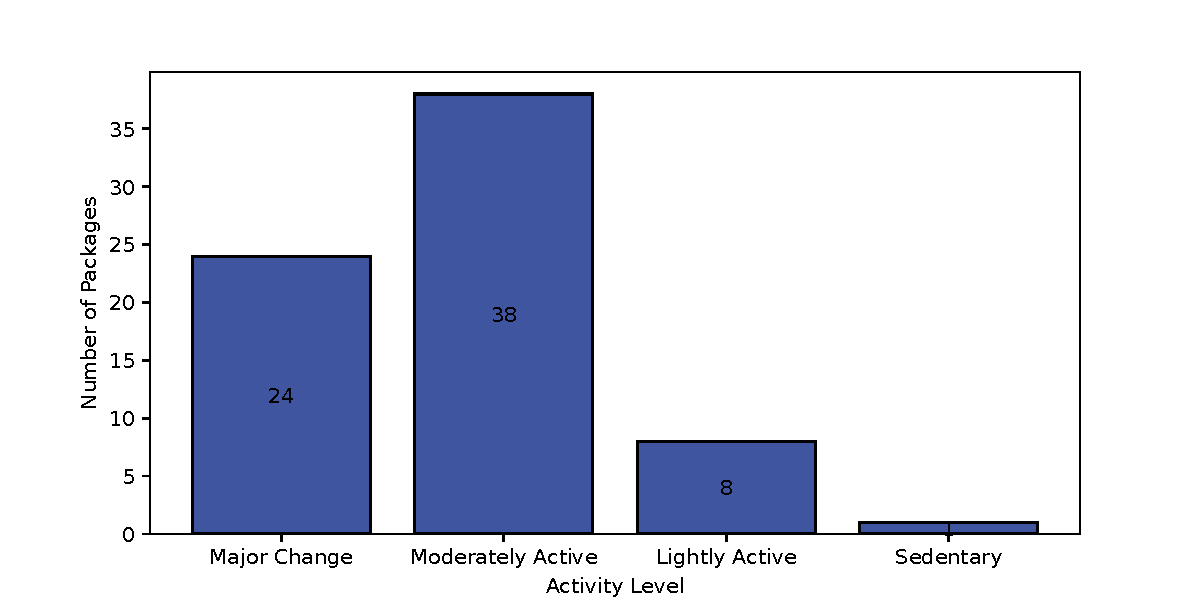
\includegraphics[width=1.0\linewidth]{figures/ubuntu-release-minimal-metadata-package-activity.pdf}
    \caption{Ubuntu Release Package Activity (minimal from R2)}
    \label{fig:ubuntu-release-minimal-metadata-package-activity}
\end{figure}


\begin{sidewaystable}[htbp]
    \centering\
    \begin{tabular}{lllll}
    \toprule
    Package & Version 14.04 & Version 22.04 & Activity & Description \\
    \midrule
    debconf & 1.5.51ubuntu2 & 1.5.79ubuntu1 & Lightly Active & Debian configuration management system \\
    libbz2-1.0 & 1.0.6-5 & 1.0.8-5build1 & Lightly Active & high-quality block-sorting file compressor library - runtime \\
    libcap-ng0 & 0.7.3-1ubuntu2 & 0.7.9-2.2build3 & Lightly Active & An alternate POSIX capabilities library \\
    libdb5.3 & 5.3.28-3ubuntu3 & 5.3.28+dfsg1-0.8ubuntu3 & Sedentary & Berkeley v5.3 Database Libraries [runtime] \\
    libdevmapper1.02.1 & 2:1.02.77-6ubuntu2 & 2:1.02.175-2.1ubuntu4 & Lightly Active & Linux Kernel Device Mapper userspace library \\
    libmnl0 & 1.0.3-3ubuntu1 & 1.0.4-3build2 & Lightly Active & minimalistic Netlink communication library \\
    mawk & 1.3.3-17ubuntu2 & 1.3.4.20200120-3 & Lightly Active & Pattern scanning and text processing language \\
    sensible-utils & 0.0.9 & 0.0.17 & Lightly Active & Utilities for sensible alternative selection \\
    zlib1g & 1:1.2.8.dfsg-1ubuntu1 & 1:1.2.11.dfsg-2ubuntu9 & Lightly Active & compression library - runtime \\
    \bottomrule
    \end{tabular}
    \caption{Lightly Active and Sedentary Packages in Ubuntu Minimal Dataset }
    \label{tab:sedentary-packages}
\end{sidewaystable}

\begin{tcolorbox}[enhanced,attach boxed title to top center={yshift=-3mm,yshifttext=-1mm}, colback=blue!5!white,colframe=blue!75!black,colbacktitle=red!80!black, title=Answer to RQ3 ,fonttitle=\bfseries, boxed title style={size=small,colframe=red!50!black} ]

We developed PVAC, a systematic method for assessing the staleness of packages within the Ubuntu main package repository.  Using this method we identified 294 packages whose upstream version had not changed in the 8-year period between the 14.04 and 22.04 releases. Using this same method, on the Minimal Dataset from RQ2 we identified 9 packages whose upstream version has had few to no changes over the 8-year evaluation period.

\end{tcolorbox}

\section{Discussion}

As stated in the title of this paper, we wanted to investigate the management and maintenance of core Ubuntu server packages. Our examination revealed compelling insights into the stability and longevity of the Ubuntu ecosystem, as measured by the libyears metric. Libyears quantifies the cumulative age of library code running in a given system, reflecting the accumulated effort invested in maintaining and refining software packages over time. Our findings demonstrate that the libyears calculations across core Ubuntu packages are indicative of sustained development efforts and ongoing maintenance.

We explored using the version number delta calculation and found that it does give valuable insight into the health of a system. We believe this insight is an important finding because the version number is the most accessible and universal way to compare packages across distributions. For example, with our method, it would be possible to calculate the libyears for Ubuntu and Fedora with version numbers alone.

In addition to libyears, we incorporated upstream release dates into our analysis to gauge the distribution's responsiveness to upstream developments and its ability to incorporate the latest features and improvements. By comparing Ubuntu package versions with their corresponding upstream releases, we assessed the timeliness of package updates and the degree of alignment with the broader software development community.

While it was surprising to find one stale package in the core Ubuntu dataset, a closer look at that package revealed that the Ubuntu package maintainers are manually applying patches to the upstream source. So, while the version number has been the same for eight years, the actual contents of the package are different. This insight could present a problem in itself as it could mislead users of the package, so we submitted a bug report reporting our findings.

\section{Threats to Validity}
In RQ1, it is likely that some packages may have been incorrectly classified due to the lack of standardized upstream versioning. For example, packages that use the date format YYYY.DD.MM was found in the place of Major.Minor.Patch. Processing this for the libyears analysis in RQ2 can cause erratic results because libyears are calculated using differences. However, the PVAC analysis presented is more robust as it examines only changes in the version fields, not the magnitude of those changes.

Also in RQ1, we found that there were changes in the upstream versioning format between Ubuntu releases, however the epoch value was not set, leading to incorrect version comparisons. This impacted the libyears analysis in RQ2 because the difference between the different versioning schemes was invalid, while in the PVAC analysis these packages were classified as highly active instead of simply being excluded. Fortunately, this does not seem to affect the results for packages with little or no activity.

In RQ3, the PVAC analysis only considers the upstream version component of the package version string and does not capture the changes made in the debian\_revision portion of the package version string as shown in Listing~\ref{lst:debian_upstream}. This could be a future research area to determine the impact that the additional data provides.

\section{Conclusion}

In conclusion, our research underscores the significance of maintaining robust software health in Ubuntu core packages and confirms that the Ubuntu community is active and engaged. Leveraging metrics such as libyears and upstream release dates provides valuable insights into the maturity, resilience, and responsiveness of the Ubuntu distribution. Moving forward, sustained vigilance, collaboration with upstream projects, and continued focus on maintaining the freshness of the packages that help run the world will have to be closely monitored. While we found only one package that has not seen any updates in 8 years in the set of core packages, we must be careful not to let that number climb.

Developing software and keeping it healthy is a complex process. There are so many variables that impact the health of a project that it is not possible to implement and monitor them all. We drilled down into one metric that was defined by the CHAOSS project and examined how to apply that metric to a complex software system. We proposed a novel way to calculate the staleness of a package based solely on the version number, which is one of the most accessible data points available in a large system such as Ubuntu.

Future work can examine how to integrate the debian\_revision tag into the calculation process in order to get a better picture of the system's health. Additionally, integrating this work into a system health dashboard for the packaging process could give better visibility to the core software that is running a large portion of the world's infrastructure. Another interesting future work direction would be to take our method of calculating the version number delta across multiple distributions. We found that the actual dates for a version can be hard to find or ambiguous. Version Numbers from upstream sources, however, are incredibly consistent and could give a better global picture.

\section{Funding Statement}
There is no funding involved in this research. 

%\bibliographystyle{plain}
\bibliography{paper}


\end{document}
